\section{Séance 6 : Choix du producteur en concurrence parfaite et monopole}


\subsection{Concurrence parfaite}
La concurrence parfaite est l'un des 4 types de marché existants. Elle est constituée de plein de petites firmes qui se font une concurrence extrêmement rude. C'est le plus intéressant, qui a la meilleure technologie, qui l'emporte. Les prix vont très bien refléter les couts de production. On ne manipule pas les prix, on ne fait qu'entrer ou sortir.


\begin{center}
	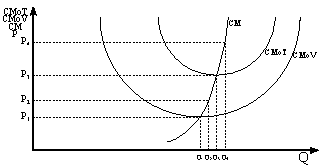
\includegraphics[height=4.5cm]{images/graph_concurrence_parfaite_court_terme.pdf}\\
	Concurrence parfaite : décision de production à court terme
\end{center}
\begin{itemize}
	\item Demande parfaitement élastique ;
	\item P$_4$/Q$_4 \Rightarrow$ Produit avec bénéfice ;
	\item P$_3$/Q$_3 \Rightarrow$ Seuil de rentabilité $\Leftrightarrow$ $P = min( CMoT )$ avec $Q$ $\Leftrightarrow$ $(CMoT)’ = 0$ ;
	\item P$_2$/Q$_2 \Rightarrow$ Produit avec perte, mais produit quand même ;
	\item P$_1$/Q$_1 \Rightarrow$ Seuil de fermeture $\Leftrightarrow$ $P = min( CMoV )$ avec $Q = 0$.
\end{itemize}

\begin{center}
	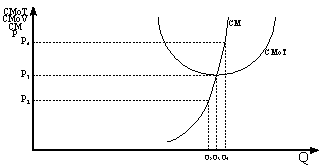
\includegraphics[height=4.5cm]{images/graph_concurrence_parfaite_long_terme.pdf}\\
	Concurrence parfaite : décision de production à long terme
\end{center}
\begin{itemize}
	\item Demande parfaitement élastique
	\item P$_4$/Q$_4 \Rightarrow$ Profit positif ;
	\item P$_3$/Q$_3 \Rightarrow$ Profit nul $\Leftrightarrow$ $P = min( CMoT )$ avec $Q$ $\Leftrightarrow$ $(CMoT)’ = 0$ ;
	\item P$_2$/Q$_2 \Rightarrow$ Profit négatif, fermeture.
\end{itemize}



\subsection{Monopole}
Le monopole est l'un des 4 types de marché existants. Elle est constituée que d'une seule firme. Soit on a une économie d'échelle tellement énorme que personne ne peut entrer et survivre, soit on a un problème légal.

Le monopole maximise son profit :
$$max( \Pi ) = RT - CT$$
$$\frac{d\Pi}{dQ} = RM - CM = 0 \Rightarrow RM = CM$$



\subsubsection{Court terme}
\begin{itemize}
	\item On produit quand $P > CMoT$
\end{itemize}



\subsubsection{Long terme}
\begin{itemize}
	\item On reste sur le marché quand $P > CMoV$
\end{itemize}

